\documentclass[a4paper,12pt]{article}

%A Few Useful Packages
\usepackage{marvosym}
\usepackage{fontspec} 					%for loading fonts
\usepackage{xunicode,xltxtra,url,parskip} 	%other packages for formatting
\RequirePackage{color,graphicx}
\usepackage[usenames,dvipsnames]{xcolor}
\usepackage[big]{layaureo} 				%better formatting of the A4 page
% an alternative to Layaureo can be ** \usepackage{fullpage} **
\usepackage{supertabular} 				%for Grades
\usepackage{titlesec}
%custom \section
\usepackage{comment}
\usepackage{amssymb}

\usepackage{makecell}
\usepackage{fontawesome}

%Setup hyperref package, and colours for links
\usepackage{hyperref}
\definecolor{linkcolour}{rgb}{0,0.2,0.6}
\hypersetup{colorlinks,breaklinks,urlcolor=linkcolour, linkcolor=linkcolour}

%FONTS
\defaultfontfeatures{Mapping=tex-text}
%\setmainfont[SmallCapsFont = Fontin SmallCaps]{Fontin}
%%% modified for Karol Kozioł for ShareLaTeX use
\setmainfont[
SmallCapsFont = Fontin-SmallCaps.otf,
BoldFont = Fontin-Bold.otf,
ItalicFont = Fontin-Italic.otf
]
{Fontin.otf}
%%%

%CV Sections inspired by: 
%http://stefano.italians.nl/archives/26
\titleformat{\section}{\Large\scshape\raggedright}{}{0em}{}[\titlerule]
\titlespacing{\section}{0pt}{3pt}{3pt}
%Tweak a bit the top margin
%\addtolength{\voffset}{-1.3cm}

%Italian hyphenation for the word: ''corporations''
\hyphenation{im-pre-se}

%-------------WATERMARK TEST [**not part of a CV**]---------------
\usepackage[absolute]{textpos}

\setlength{\TPHorizModule}{35mm}
\setlength{\TPVertModule}{\TPHorizModule}
\textblockorigin{2mm}{0.65\paperheight}
\setlength{\parindent}{0pt}

%--------------------BEGIN DOCUMENT----------------------
\begin{document}

%WATERMARK TEST [**not part of a CV**]---------------
%\font\wm=''Baskerville:color=787878'' at 8pt
%\font\wmweb=''Baskerville:color=FF1493'' at 8pt
%{\wm 
%	\begin{textblock}{1}(0,0)
%		\rotatebox{-90}{\parbox{500mm}{
%			Typeset by Alessandro Plasmati with \XeTeX\  \today\ for 
%			{\wmweb \href{http://www.aleplasmati.comuv.com}{aleplasmati.comuv.com}}
%		}
%	}
%	\end{textblock}
%}

\pagestyle{empty} % non-numbered pages

\font\fb=''[cmr10]'' %for use with \LaTeX command
\vspace{3mm}
\begin{tabular}{rl}
\smash{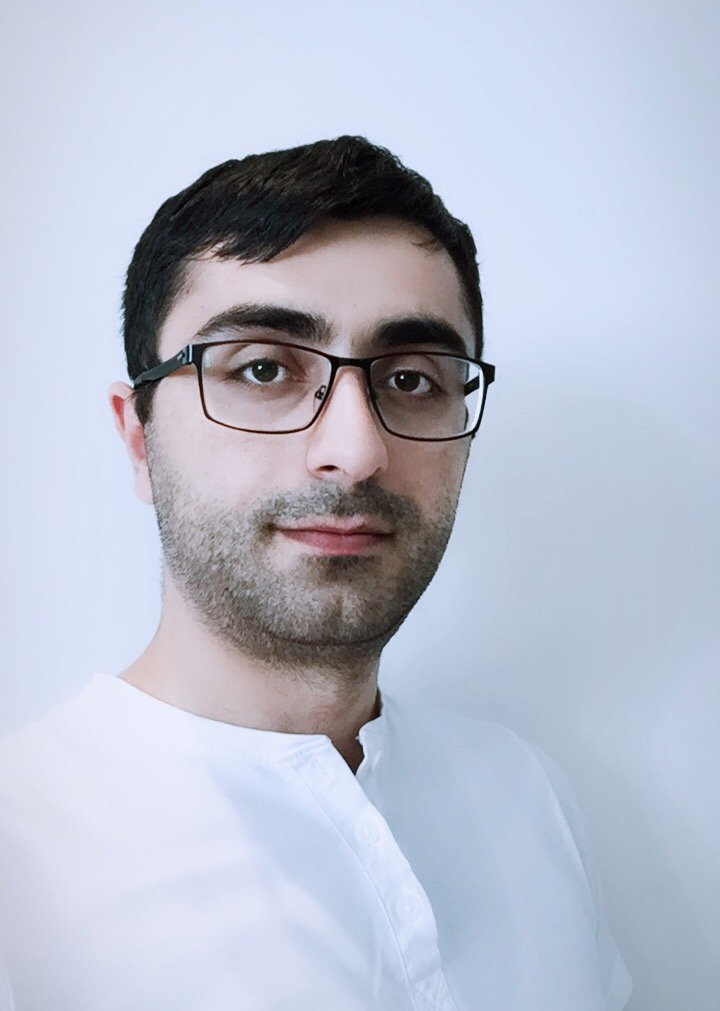
\includegraphics[width=4cm]{image1.JPG} }&
\raisebox{90pt}
		{\Huge \hspace{20mm} Gevorg \hspace{1mm}Minasyan} 

\end{tabular}
%--------------------SECTIONS-----------------------------------
%Section: Personal Data

\vspace{4mm}
\section{Personal Data}

\begin{tabular}{rl}
    \vspace{1mm}
    \textsc{Place and Date of Birth:} & Vardenis, Armenia  | 19 Apr 1994 \\
    
    \vspace{1mm}
    \textsc{Address:}   & Andranik str. 68, apt. 38, Yerevan, Armenia \\
    
        \vspace{1mm}
    \textsc{Phone:}     & +374 94 208660\\
        \vspace{1mm}
    \textsc{email:}     & \href{mailto:gevor.minasyan94@gmail.com}{gevor.minasyan94@gmail.com}\\
        \vspace{1mm}
    \textsc{github:}    & 
    \href{https://github.com/Gevorg-Minasyan}{\Large{\faGithub}} \\
         \textsc{linkedin:}    &  \href{https://www.linkedin.com/in/gevorg-minasyan-42475a132/}{\Large{\faLinkedin}}
\end{tabular}
%Section: Work Experience at the top
\section{Work Experience}

\begin{tabular}{r|p{12.2cm}}
 \emph{Current} & Data Scientist and ML/DL Specialist at \textsc{Intent.ai}, Yerevan \\\textsc{Jun 2018}&\emph{Adtech, Software} \\\cline{2-2}& \\& \emph{Projects and Tasks:}\\&\footnotesize{
 \begin{itemize}
  \item Design and implementation of demographic attribute prediction system.
  \item Design and implementation of website classification system.
  \item Integrating DL models with apache spark
  \item Visualizing data to help with evaluating algorithms and producing regular reports.
\end{itemize}}\\\multicolumn{2}{c}{} 
\end{tabular}

\begin{tabular}{r|p{12.2cm}}
 \emph{Current} & Data Scientist and ML/DL Specialist at \textsc{Ucom LLC}, Yerevan \\\textsc{Sep 2017}&\emph{Internet and Telecommunications Service Provider} \\\cline{2-2}& \\& \emph{Projects and Tasks: }\\&\footnotesize{
 \begin{itemize}
 \item Design and build production-ready machine-learning models.
  \item Building tools and methods for looking into the cleanliness of data.
  \item Extracting distributed unsupervised representations from dns log.
  \item Extracting distributed unsupervised representations from cdr log.
  \item Design and implementation of credit scoring system.

\end{itemize}}\\\multicolumn{2}{c}{} 
\end{tabular}

\begin{tabular}{r|p{12.2cm}}
 \textsc{Apr 2017} & Software Engineer at \textsc{Synergy Int. Systems}, Yerevan \\\textsc{Sep 2015}&\emph{Software Development}  \\ \cline{2-2}& \\& \emph{Tasks include: }\\& \footnotesize{
 \begin{itemize}
  \item Design and implementation of large data entries using java and related technologies.
  \item Develop cross-browser web applications in object-oriented approach.
  \item Working experience with relational database.
  \item Able to correct software defects and make updates on an existing software.
\end{itemize}}\\
\multicolumn{2}{c}{} \\
\end{tabular}

%Section: Education
\section{Education}
\begin{tabular}{rl}	
 \emph{Current} & Master of Science in \textsc{Numerical Analysis} and \textsc{Mathematical Modelling}, \\\textsc{Sep} 2017&\normalsize\textbf{Yerevan State University}, Yerevan\\

& Thesis: \makecell { ``\href{https://github.com/Gevorg-Minasyan/master-thesis}{On Generalization Error Bound Estimation of  }\\  \href{https://github.com/Gevorg-Minasyan/master-thesis}{Certain Transform Learning Method}'' } \\& \small Advisor: Hayk E. \textsc{Danoyan} \\
&\normalsize \textsc{Gpa}: 20/20%\hyperlink{grds}{\hfill | \footnotesize Detailed List of Exams}
\\&\\
\textsc{2012 - 2017} & Bachelor of Science in \textsc{Applied Mathematics} and \textsc{Informatics}, \\& \normalsize\textbf{Yerevan State University}, Yerevan\\
& Thesis: ``\href{https://arxiv.org/pdf/1912.01546.pdf}{On the Deficiency of Complete Multi-partite Graphs}'' \\& \small Advisor:   \textsc{Petros A. Petrosyan}\\
&\normalsize \textsc{Gpa}: 19.22/20%\hyperlink{grds_cleli}{\hfill| \footnotesize Detailed List of Exams}
\end{tabular}

%Section: Trainings and additional info
\vspace{5mm}
\section{Trainings and Certificates}
\begin{tabular}{rl}
% \textsc{Jul} 2015 – \textsc{Aug} 2015 & Scholarship for graduate students with an outstanding curriculum \footnotesize(\EURcr 30,000)\normalsize\\
 \textsc{Jul} 2015 – \textsc{Aug} 2015 & Summer school courses in Synergy Int. Systems\\
 %\textsc{Nov} 2016 – \textsc{Mar} 2017 & Machine learning training course in PicsArt\\
 \textsc{Apr} 2017 – \textsc{Aug} 2017 & Machine learning and data science training course in ACA %(\EyesDollar 3,000)\normalsize\\
\end{tabular}

\vspace{5mm}
\section{TECHNICAL SKILLS}
\begin{tabular}{rl}
\textbf{Machine Learning:}& classification, regression, clustering, convnets, \\ &object detection, object tracking, \\ & unsupervised representation learning \\& topic modeling \\
\textbf{Statistical Methods:}& time series,  A/B testing, density estimation \\
\textbf{Software and Programming Languages:}& Python (scikit-learn, numpy, scipy, pandas) \\&
Flask, TensorFlow, PyTorch, Keras, 
PySpark, \\& Hadoop,  MongoDB, JAVA, SQL,  {\fb \LaTeX}, GIT, Docker\\
\end{tabular}
\newpage
\section{RECOGNIZED ACHIEVEMENTS}
Smart City Hackathon 2017\\
Hackathon Organizers:  Yerevan Municipality, Kolba Lab\\
Team: \textsc{Datathon} \\
Achievements and Awards:\\ 
\vspace{-5mm}
\begin{itemize}
\item[$\checkmark$] \textbf{2\textsuperscript{nd} Winner Award}
\item[$\checkmark$] \textbf{Certificate of Achievement}
\end{itemize}


%Section: Languages
\section{Languages}
\begin{tabular}{rl}
 \textsc{Armenian:}&Mothertongue\\
\textsc{English:}&Good Working Knowledge\\
\textsc{Russian:}&Basic Knowledge\\
\end{tabular}

\section{Interests and Activities}
Football, Reading, Swimming



\end{document}
